%%%%%%%%%%%%%%%%%%%%%%%%%%%%%%%%%%%%%%%%%%%%%%%%%%%%%%%%%%%%%%%%%%%%%%%%%%%%%%%%
\chapter{Νευρομυοσκελετικό Σύστημα}

Σε αυτό το κεφάλαιο παρουσιάζουμε την διαδικασία της ορθής δυναμικής σε νευρομυοσκελετικά μοντέλα. Στόχος είναι να εκτιμηθούν οι δυνάμεις που παράγονται από τους μύες, που μετατρέπονται σε  ροπές, οι οποίες με την σειρά τους σε κίνηση που προήρθε από την νευρική διέγερση των μυών. Η παραπάνω διαδικασία μπορεί να χωριστεί σε τέσσερα βήματα, την μυϊκή ενεργοποίση (\eng{muscle activation dynamics}), την μυϊκή συστολή (\eng{muscle contraction dynamics}), την μυοσκελετική γεωμετρία και τέλος την εξίσωσης της κίνησης, η οποία επιτρέπει την μετατροπή της ροπής των αρθρώσεων σε κίνηση.

%%%%%%%%%%%%%%%%%%%%%%%%%%%%%%%%%%%%%%%%%%%%%%%%%%%%%%%%%%%%%%%%%%%%%%%%%%%%%%%%
\section{H Φυσιολογία του Μυ}

%%%%%%%%%%%%%%%%%%%%%%%%%%%%%%%%%%%%%%%%%%%%%%%%%%%%%%%%%%%%%%%%%%%%%%%%%%%%%%%%
\subsection{Δομή}

Ο σκελετικός μυς είναι μια συλλογή από μυϊκά κύτταρα (μυϊκές ίνες) \cite{zirinoglou}. Ο αριθμός των μυϊκών ινών εξαρτάται από το μέγεθος του μυός και ποικίλει από μερικές εκατοντάδες έως αρκετές χιλιάδες ίνες. Ολόκληρος ο μυς καλύπτεται και προστατεύεται από ένα συνδετικό περιτοναϊκό ιστό, ο όποιος περιβάλλει κάθε μυϊκή ίνα, τένοντα, οστό, νεύρο και αγγείο. Ο μυς διαιρείται περεταίρω σε αρκετές μυϊκές δεσμίδες. Κάθε δέσμη περιέχει περίπου εκατό μυϊκές ίνες. Κάθε ίνα έχει διάμετρο 50μ\eng{m} με 100μ\eng{m} (χιλιοστά του χιλιοστόμετρου), μήκος 2 με 6 εκατοστά και περιέχει περισσότερα από 1000μ\eng{m} με 2000μ\eng{m} μυϊκά ινίδια, τα οποία με την σειρά τους περιέχουν μια αλυσίδα από σαρκομέριο. Κάθε μυϊκό ινίδιο αποτελείται από αρκετούς τύπους πρωτεϊνών.

\begin{figure}[H]
    \centering
    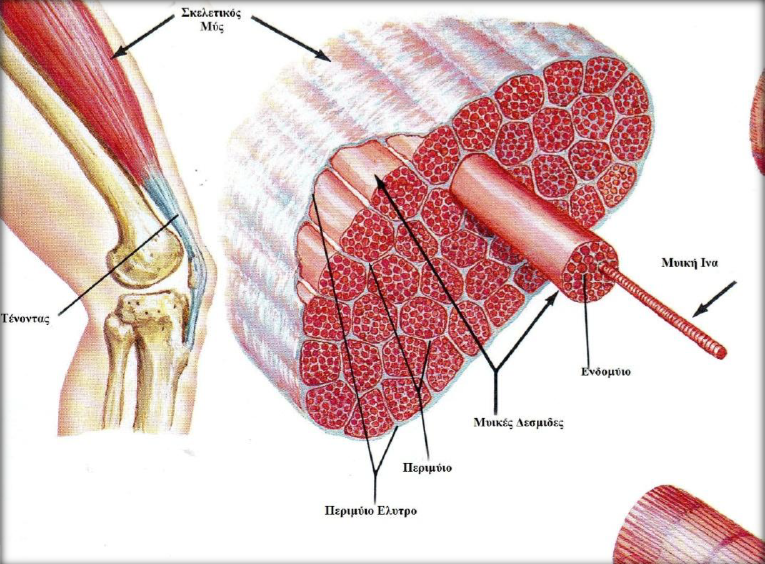
\includegraphics[width=.7\textwidth]{neuromusculoskeletal/fig/muscle-fysiology.png}
    \caption{Σκελετικός μυς: ανατομική περιγραφή\protect\footnotemark}
    \label{fig:muscle-fysiology}
\end{figure}


\begin{figure}[H]
    \centering
    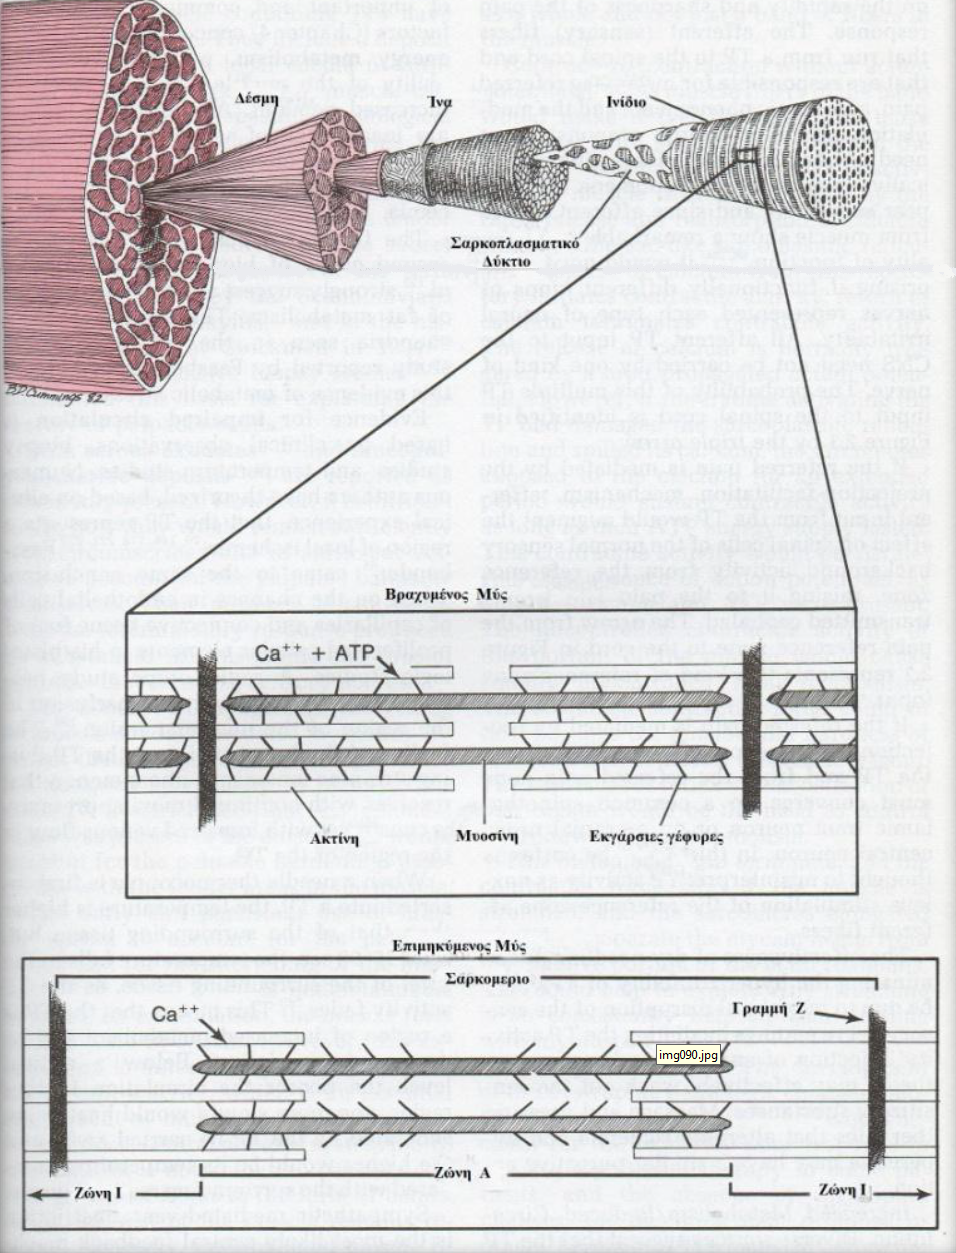
\includegraphics[width=.7\textwidth, height=0.5\textheight]{neuromusculoskeletal/fig/muscle-fysiology2.png}
    \caption{Δομή και συσταλτικός μηχανισμός του φυσιολογικού σκελετικού μυός\protect\footnotemark}
    \label{fig:muscle-fysiology2}
\end{figure}
\footnotetext{Εικόνα από το βιβλίο \eng{Travell \& Simons} 1999}

Τo σαρκομέριο είναι η συσταλτή μονάδα του μυϊκού ινιδίου και αποτελείται από επικαλυπτόμενες εγκάρσιες γέφυρες ακτίνης και μυοσίνης. Το σαρκομέριο δίνει την δυνατότητα στον μυ να συσπάται και να χαλαρώνει. Όταν ο μυς συσπάται, τα λεπτά νημάτια ακτίνης και μυοσίνης ολισθαίνουν μεταξύ τους και ο μυς βραχύνεται. Όταν ο μυς χαλαρώνει, οι εγκάρσιες γέφυρες ολισθαίνουν ήπια και ξεχωριστά, και ο μυς επιστρέφει στο μήκος ηρεμίας.

\begin{figure}[H]
    \centering
    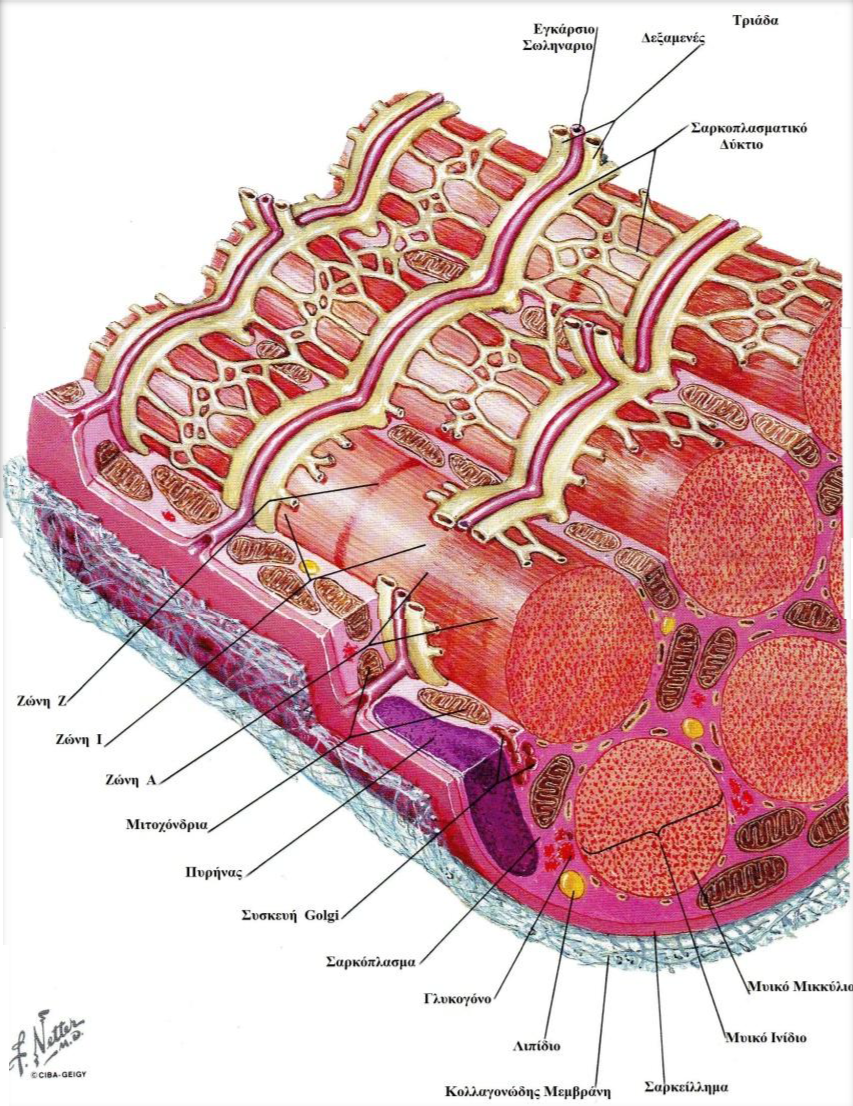
\includegraphics[width=.7\textwidth, height=0.6\textheight]{neuromusculoskeletal/fig/muscle-fysiology3.png}
    \caption{Σαρκοπλασματικό δίκτυο\protect\footnotemark}
    \label{fig:muscle-fysiology3}
\end{figure}
\footnotetext{Εικόνα από το βιβλίο \eng{Netter} 1987}

%%%%%%%%%%%%%%%%%%%%%%%%%%%%%%%%%%%%%%%%%%%%%%%%%%%%%%%%%%%%%%%%%%%%%%%%%%%%%%%%
\subsection{Σαρκοπλασματικό Δίκτυο}

Το σαρκοπλασματικό (\eng{Kandel E.et al} 2000, \eng{Fawcett D} 1986) δίκτυο είναι ένα δίκτυο σωληνοειδούς μορφής το οποίο εκτείνεται σε ολόκληρο τον μυ. Τα επιμήκη σαρκοπλασματικά σωληνάρια καταδύονται σε μια σχετικά μεγάλη τελική δεξαμενή σε οποιαδήποτε άκρη του σαρκομερίου. Δυο τελικές δεξαμενές σε συνδυασμό με ένα εγκάρσιο σωληνάριο(\eng{T-tubule}) σχηματίζουν μια τριάδα (\eng{Silverthorn D} 1998). Η τριάδα είναι τοποθετημένη σε καίρια θέση δίπλα από το τμήμα της μυϊκής ίνας, το οποίο παράγει τις απαραίτητες δυνάμεις για την συστολή. Το εγκάρσιο σωληνάριο παίζει ένα σημαντικό ρόλο στη διέλευση του δυναμικού ενέργειας βαθιά μέσα στον μυ. Ο ρόλος του σαρκοπλασματικου δικτύου είναι να αποθηκεύει $Ca^{2+}$, το οποίο είναι απαραίτητο για την συστολή του μυός.

%%%%%%%%%%%%%%%%%%%%%%%%%%%%%%%%%%%%%%%%%%%%%%%%%%%%%%%%%%%%%%%%%%%%%%%%%%%%%%%%
\subsection{Το Νευρικό Σύστημα}

Η κύρια εργασία του κινητικού νευρικού συστήματος είναι να ελέγχει και να συντονίζει τη λειτουργία των συσταλτών στοιχείων σε όλους τους μύες ταυτόχρονα, έτσι ώστε να εφαρμόζεται η κατάλληλη τάση στον σκελετό για να παραχθεί η επιθυμητή κίνηση (\eng{Kandel et al} 200).

\begin{figure}[H]
    \centering
    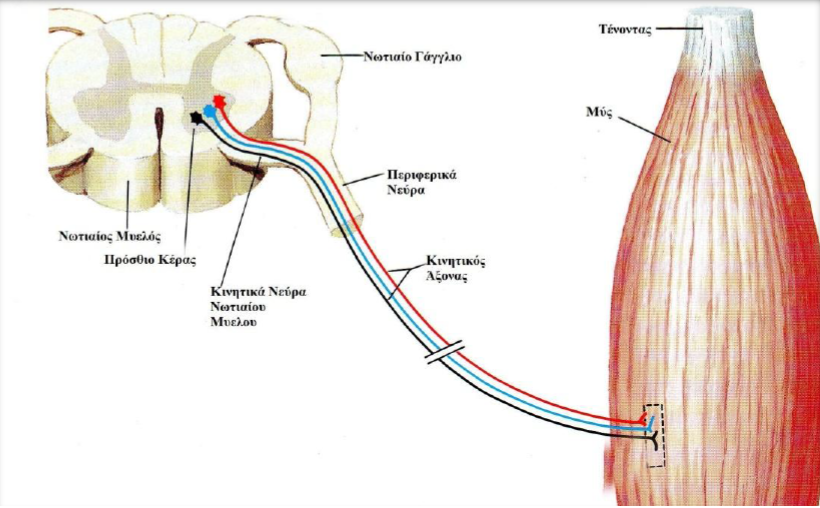
\includegraphics[width=.8\textwidth]{neuromusculoskeletal/fig/muscle-fysiology4.png}
    \caption{Κινητικοί νευρώνες του νωτιαίου μυελού\protect\footnotemark}
    \label{fig:muscle-fysiology4}
\end{figure}
\footnotetext{Εικόνα από το βιβλίο \eng{Netter} 1987}

Ο κινητικός νευρώνας θεωρείται ως η λειτουργική μονάδα του κινητικού νευρικού συστήματος. Τα κυτταρικά σώματα των κινητικών νευρώνων είναι στοιβαγμένα σε έναν κινητικό πυρήνα μέσα στο κοιλιακό τμήμα της σπονδυλικής στήλης. Ο άξονας κάθε κινητικού νευρώνα εκφύεται από την σπονδυλική στήλη διαμέσου μιας κοιλιακής ρίζας (ή ενός κρανιακού νεύρου από το εγκεφαλικό στέλεχος) και διαιρείται σε μικρότερους κλάδους περιφερικών νεύρων μέχρι να εισέλθει στον μυ που ελέγχεται από αυτό το νεύρο. Οι άξονες των κινητικών νευρώνων είναι εμμύελοι. Δύνανται έτσι να μεταδίδουν δυναμικά ενέργειας με υψηλή ταχύτητα, επιτρέποντας ώσεις από το κεντρικό νευρικό σύστημα να μεταφέρονται στις μυοσκελετικές ίνες με ελάχιστη καθυστέρηση. Με την άφιξη του στο μυ, ο άξονας του κινητικού νευρώνα διακλαδίζεται πολλαπλά, με κάθε διακλάδωση να σχηματίζει μια απλή σύναψη με μια μυϊκή ίνα.

Το απόλυτο μυϊκό μήκος και οι αλλαγές του μυϊκού μήκους ανιχνεύονται από διατατικούς αισθητήρες που είναι στρωμένοι μέσα στο μυ. Οι αισθητήρες αυτοί αποτελούνται από απολήξεις προσαγωγών νευρικών ινών που είναι τυλιγμένες γύρω από τροποποιημένες μυϊκές ίνες, αυτή η δομή ονομάζεται μυϊκή άτρακτος. Είναι απαραίτητες για την γνώση της θέσης και της κίνησης των μελών, αλλά επίσης συντελεί στο λεπτό κινητικό έλεγχο.

\begin{figure}[H]
    \centering
    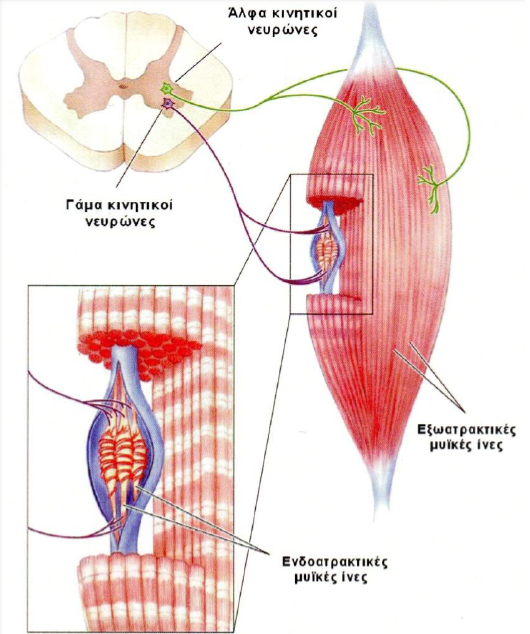
\includegraphics[width=.8\textwidth]{neuromusculoskeletal/fig/muscle-fysiology5.png}
    \caption{Κινητική μονάδα (μυϊκή άτρακτος)}
    \label{fig:muscle-fysiology5}
\end{figure}

Οι τροποποιημένες μυϊκές ίνες που ένγκεται μέσα στην άτρακτο είναι γνωστές ως ενδοατράκτικες ίνες, ενώ οι μυοσκελετικές ίνες, οι οποίες αποτελούν την πλειονότητα των ινών ενός μυός και παράγουν δύναμη και κίνηση, ονομάζονται εξωατράκτιες ίνες. Μέσα στην μυϊκή άτρακτο υπάρχουν δύο διατατικοί αισθητήρες. Το ένα είδος ανταποκρίνεται άριστα στο πόσο ο μυς έχει διαταθεί και το άλλο στο μέγεθος και στην ταχύτητα διάτασης. Πρωταγωγείς (τύπου Ια) και δευτεραγωγείς (τύπου ΙΙ) κεντρομόλες ίνες ανέρχονται από τις μυϊκές ατράκτους, συνάπτονται με άλφα ή γάμα κινητικούς νευρώνες αντίστοιχα και διευκολύνουν τη σύσπαση των εξωατρακτικων και ενδοατρακτικων ινών.

%%%%%%%%%%%%%%%%%%%%%%%%%%%%%%%%%%%%%%%%%%%%%%%%%%%%%%%%%%%%%%%%%%%%%%%%%%%%%%%%
\subsection{\texorpdfstring{Το Αισθητήριο Όργανο \eng{Golgi}}{}}

Το όργανο του \eng{Golgi} βρίσκεται κοντά στην μυοτενόντια σύναψη, τυλίγεται γύρω από τα άκρα των εξωατρακτικών ινών του μυός και είναι ευαίσθητο στην τάση που προκαλείται στον μυ από παθητική διάταση ή από ενεργητική σύσπαση του. Το όργανο του \eng{Golgi} είναι ένας προστατευτικός μηχανισμός που αναστέλλει την σύσπαση του μυός στον όποιο βρίσκεται. Η ουδός πυροδότησης είναι πολύ χαμηλή (ενεργοποιείται εύκολα), μετά από ενεργητική μυϊκή σύσπαση και πολύ υψηλή, μετά από μια παθητική διάταση. Όταν αναπτύσσεται υπερβολική τάση στον μυ, το όργανο του \eng{Golgi} πυροδοτεί, αναστέλλει τη δραστηριότητα του άλφα κινητικού νευρώνα και μειώνει την τάση του μυός. Κατά την διάρκεια των διαδικασιών της διάτασης, η τάση στον τένοντα καθορίζει αν το κάθε σαρκομέριο του μυός είναι επιμηκυμένο.

Κατά την διάρκεια όμως της ισοτονικής και της ισομετρικής συστολής του μυός η κατάσταση διαφοροποιείται. Ενώ σταματά να διατείνεται η μυϊκή άτρακτος, το τενόντιο όργανο συνεχίζει να βρίσκεται σε διάταση και στην πραγματικότητα ο ρυθμός της πυροδότησης του αυξάνεται σε όλη τη διάρκεια της συστολής. Ο δυναμικός κώδικας του ενάντιου οργάνου σηματοδοτεί το ρυθμό αύξησης της έντασης κατά την διάρκεια της συστολής και το ρυθμό της μείωσης της διέγερσης κατά την διάρκεια της χαλάρωσης. Το πρότυπο διέγερσης των τενόντιων οργάνων κατά την διάρκεια της συστολής δείχνει ότι ο κύριος ρόλος τους είναι να ελέγχουν το ρυθμό της αλλαγής της έντασης σε έναν συστελλόμενο μυ καθώς σηματοδοτούν το ποσοστό της έντασης που υπάρχει σε έναν ισομετρικά συστελλόμενο μυ.

%%%%%%%%%%%%%%%%%%%%%%%%%%%%%%%%%%%%%%%%%%%%%%%%%%%%%%%%%%%%%%%%%%%%%%%%%%%%%%%%
\section{Μοντέλο του Μυ}

Ένα μοντέλο του μυ περιγράφει την διαδικασία παραγωγής της δύναμης κάτω από μια νευρική διέγερση και μπορούν να καταταχθούν σε μικροσκοπικά και μακροσκοπικά μοντέλα. Τα μικροσκοπικά μοντέλα ανήκουν στην κατηγορία \eng{Huxley-type} προς τιμή του \eng{Huxley 1957}, ενώ το πιο διάσημο μακροσκοπικό μοντέλο είναι το \eng{Hull-type} προς τιμή του \eng{Hill 1938}. Τα δύο αυτά μοντέλα χρησιμοποιούνται ευρέως στην επιστημονική κοινότητα. Όσον αφορά τα μοντέλα \eng{Hill-type} είναι καταλληλότερα σε εφαρμογές προσομοίωσης, γιατί είναι πιο απλά και έχουν λιγότερους παραμέτρους που πρέπει να προσδιορισθούν. Για αυτό το λόγο, η ανάλυση που θα γίνει στην συνέχεια αφορά την δεύτερη κατηγορία μοντέλων.

%%%%%%%%%%%%%%%%%%%%%%%%%%%%%%%%%%%%%%%%%%%%%%%%%%%%%%%%%%%%%%%%%%%%%%%%%%%%%%%%
\subsection{Μοντέλο Ενεργοποίησης}

Η αλληλεπίδραση μεταξύ ινιδίων μυοσίνης και ακτίνης ενεργοποιείται, όταν το μυϊκό κύτταρο δεχτεί ένα κατάλληλο σήμα από το νευρικό σύστημα. Το σήμα πυροδοτεί ένα δυναμικό ενέργειας στην κυτταρική μεμβράνη του κυττάρου. Αυτή η ηλεκτρική διέγερση διαδίδεται κατά μήκος μιας σειράς μεμβρανικών σωλήνων, τα εγκάρσια σωληνάρια, και το σήμα μεταφέρεται στο σαρκοπλασματικό δίκτυο, το οποίο περιέχει υψηλή συγκέντρωση ασβεστίου. Σαν αντίδραση στην εισερχόμενη ηλεκτρική διέγερση, μεγάλο ποσό $Ca^{+2}$ απελευθερώνεται στο κυτταροδιάλυμα μέσω ιοντικών διαύλων της μεμβράνης του σαρκοπλασματικού δικτύου που ανοίγουν εξαιτίας της ηλεκτρικής διέγερσης.

Το ιόν του ασβεστίου αλληλεπιδρά με εξειδικευμένες πρωτεΐνες που συνδέονται ισχυρά με τα ινίδια ακτίνης. Μια από αυτές τις πρωτεΐνες είναι η τροπομυοσίνη, ένα άκαμπτο ραβδόμορφο πρωτεϊνικό μόριο που προσδένεται στο αυλάκι της έλικας της ακτίνης και δεν την αφήνει να αντιδράσει με τις κεφαλές μυοσίνης. Η άλλη είναι η τροπονίνη, ένα πρωτεϊνικό σύμπλοκο που περιλαμβάνει μια πρωτεΐνη ευαίσθητη στο ασβέστιο, την τροπονίνη \eng{C}. Όταν αυξηθεί η συγκέντρωση του ασβεστίου στο κυτταροδιάλυμα, το ιόν ασβεστίου προσδένεται στη τροπονίνη και προκαλεί μια αλλαγή στο σχήμα της και έτσι οι κεφαλές μυοσίνης μπορούν να προσδεθούν στο ινίδιο ακτίνης και να αρχίσει η συστολή.

Η αύξηση του $Ca^{+2}$ στο κυτταροδιάλυμα σταματά αμέσως μετά τη διακοπή του νευρικού σήματος, επειδή το ιόν του ασβεστίου αντλείται γρήγορα πίσω στο σαρκοπλασματικό δίκτυο. Μόλις η συγκέντρωση ασβεστίου επανέλθει σε επίπεδα ηρεμίας, η τροπονίνη και η τροπομυοσίνη επιστρέφουν στις αρχικές τους θέσεις και σταματούν τη συστολή.

Ένας μυς δεν μπορεί να παράξει δύναμη ή να χαλαρώσει ακαριαία. Πειραματικά έχει αποδειχτεί ότι η καθυστέρηση από την στιγμή της διέγερσης μέχρι την ανάπτυξη της δύναμης ξεκινά από 5\eng{ms} για την παραγωγή της δύναμης από τους γρήγορους μύες του οφθαλμού, και από 40\eng{ms} έως 50\eng{ms} από μύες με πιο μεγάλα ποσοστά βραδείας σύσπασης \cite{zajac89}. Η διαδικασία της χαλάρωσης είναι πιο αργή με αποτέλεσμα να χρειαστεί περισσότερο χρόνο. Η ενεργοποίηση των μυών μπορεί να μοντελοποιηθεί με μια διαφορική εξίσωση πρώτης τάξεως.

\begin{equation}
    \begin{gathered}
        \hat{a} = \frac{a - a_{min}}{1 - a_{min}}\\[10pt]
        \frac{da}{dt} = \frac{u - \hat{a}}{\tau (\hat{a}, u)}\\[10pt]
        \tau (\hat{a}, u) =
        \begin{cases}
            t_{act} \cdot (0.5 +1.5 \cdot \hat{a}), & u > \hat{a} \\
            t_{deact}/(0.5 +1.5 \cdot \hat{a}), & u \leq \hat{a}
        \end{cases}
    \end{gathered}
    \label{equ:activation-dynamics}
\end{equation}

Όπου $u$ η διέγερση και $a$ η ενεργοποίηση. Το παραπάνω μοντέλο παρουσιάστηκε από \cite{millard13} και ακολουθεί με μικρές αλλαγές τα μοντέλα \cite{thelen03, winters95}, όπου η χρονική μεταβολή $\frac{da}{dt}$ ισούται με την διαφορά $u - a$ δια μια συνάρτηση. Η διαφορά του μοντέλου από τα προηγούμενα είναι ο παράγοντας $\hat{a}$ που κάνει την εξίσωση \ref{equ:activation-dynamics} κατάλληλη για προσομοιώσεις, κρατώντας το αποτέλεσμα στα όρια $(0.01, 1), a_{min} = 0.01$.

%%%%%%%%%%%%%%%%%%%%%%%%%%%%%%%%%%%%%%%%%%%%%%%%%%%%%%%%%%%%%%%%%%%%%%%%%%%%%%%%
\subsection{Μοντέλο Συστολής}

Αφότου έχει εκτιμηθεί η ενεργοποίση \eng{a} του μυ, το επόμενο βήμα είναι ο προσδιορισμός της δύναμης που θα παράξει. Όπως αναφέραμε τα μοντέλα \eng{Huxley-type} περιγράφονται από πολύπλοκες εξισώσεις, με πολλούς παραμέτρους, που πρέπει στην πορεία της προσομοίωσης να ολοκληρωθούν, με αποτέλεσμα να έχουν μεγάλο υπολογιστικό κόστος. Για αυτούς τους λόγους, θα περιγράψουμε τα μοντέλα \eng{Hill-type}.

\begin{figure}[H]
    \centering
    \begin{subfigure}[Η]{.5\textwidth}
        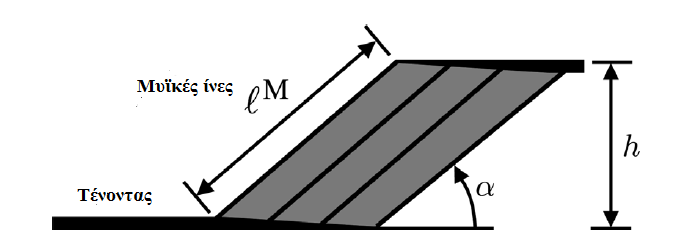
\includegraphics[width=\textwidth]{neuromusculoskeletal/fig/simple-muscle-model.png}
        \caption{Απλοποιημένο μοντέλο\cite{millard13}}
        \label{fig:simple-mascle-model}
    \end{subfigure} ~
    \begin{subfigure}[Η]{.4\textwidth}
        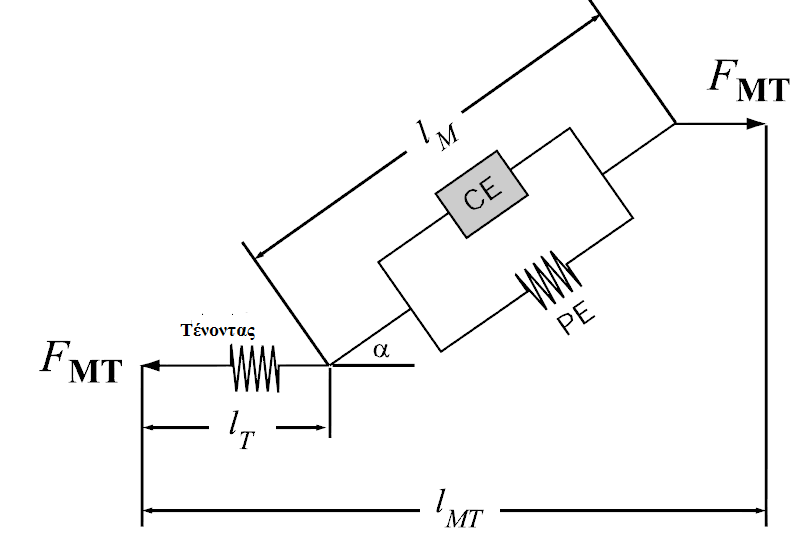
\includegraphics[width=\textwidth]{neuromusculoskeletal/fig/muscle-model.png}
        \caption{Μαθηματικό μοντέλο\cite{erdemir07}}
        \label{fig:muscle-model}
    \end{subfigure}
    \caption{Μοντέλο του μυ}
\end{figure}
%\footnotetext{Εικόνες από την δημοσίευση \cite{millard13}}

Όπως φαίνεται στην εικόνα \ref{fig:simple-mascle-model} οι μυικές ίνες συνδέονται με τον τένοντα υπό μια γωνιά α (\eng{pennation angle}). Η μοντελοποίηση της συστολής αποτελείται από τρία μέρη: το παθητικό (\eng{passive element}) που είναι μια δύναμη που ασκείται όταν ο μυς τεντωθεί πάνω από ένα συγκεκριμένο όριο, ο συστολικός μηχανισμός (\eng{contractile element}) που αφορά την παραγωγή της κύριας μυικής δύναμης και το σειριακό μέρος που έχει να κάνει με τις δυνάμεις που ασκούνται από το τένοντα.

Πριν περιγράψουμε τις συναρτήσεις, μπορούμε να δούμε την καμπύλη κανονικοποιημένης δύναμης σε σχέση με το μήκος του μυ \ref{fig:active-force-legnth}. Στον άξονα \eng{x} έχουμε το κανονικοποιημένο μήκος με βάση το βέλτιστο μήκος του μυ $l^{M}_{o}$ (\eng{optimal fiber length}), ενώ στο άξονα \eng{y} έχουμε την κανονικοποιημένη δύναμη με βάση την μέγιστη ισομετρική δύναμη $f^{M}_{o}$ (\eng{maximum isometric force}). Οι καμπάνες συμβολίζουν την δύναμη που παράγει ο μυς και διαφοροποιούνται για διαφορετικές τιμές ενεργοποίησης \eng{a}, που κυμαίνονται από $a_{min}$ μέχρι 1. Όταν το μήκος του μυ βρίσκεται σε μικρότερη ή μεγαλύτερη τιμή από την $l^{M}_{o}$ δεν μπορεί να παράξει την μέγιστη δύναμη, εξαιτίας της μειωμένης επικάλυψης μεταξύ της ακτίνης και της μυοσίνης. Πρέπει να προσέξουμε ότι το βέλτιστο της καμπάνας δεν βρίσκεται για $l = 100\%$ όσο μειώνεται η τιμή του \eng{a}. Επίσης, βλέπουμε ότι όταν ξεπεράσουμε ένα όριο επιμήκυνσης εμφανίζεται μια εκθετική δύναμη, που συμβολίζει την παθητική λειτουργία του μυ. Τέλος, η σύνθεση των δύο δυνάμεων παράγουν την καμπύλη δύναμη-μήκους για δεδομένη διέγερση.

\begin{figure}[H]
    \centering
    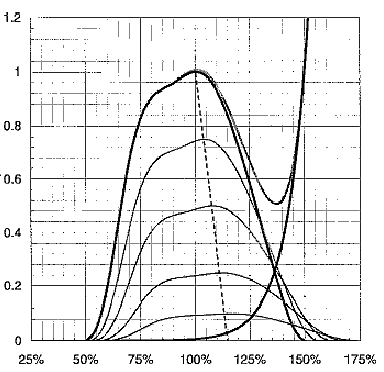
\includegraphics[width=.5\textwidth, height=.35\textheight]{neuromusculoskeletal/fig/active-force-legnth.png}
    \caption{Καμπύλη δύναμη-μήκους για διαφορετικές τιμές ενεργοποιήσης\cite{buchanan04}}
    \label{fig:active-force-legnth}
\end{figure}
%\footnotetext{Εικόνα από την δημοσίευση \cite{buchanan04}}

\begin{figure}[H]
    \centering
    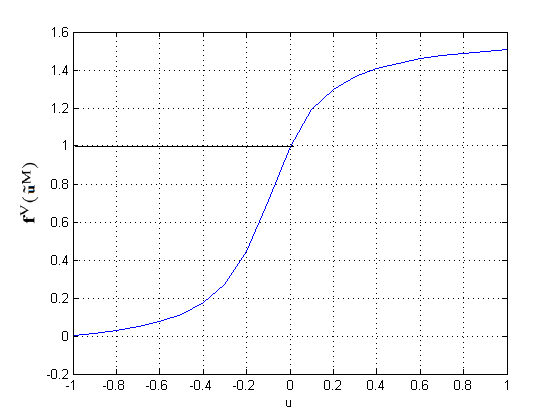
\includegraphics[width=.6\textwidth]{neuromusculoskeletal/fig/force-velocity.png}
    \caption{Καμπύλη δύναμη-ταχύτητας}
    \label{fig:force-velocity}
\end{figure}
%\footnotetext{Εικόνα από την δημοσίευση \cite{millard13}}

Πέραν της σχέσης δύναμης-μήκους έχουμε και έναν άλλο παράγοντα που συνεισφέρει και σχετίζεται με την καμπύλη δύναμης-ταχύτητας \ref{fig:force-velocity}. Αυτή η δύναμη μοντελοποιεί την μη γραμμικότητα του ρυθμού επιμήκυνσης ή συστολής. Η δύναμη που παράγεται από τον μυ δίνεται από την εξίσωση της δύναμης.

\begin{equation}
    f^{M} = f^{M}_{o} \cdot (a \cdot f^{L}(\tilde{l}^{M}) \cdot f^{V}(\tilde{v}^{M}) + f^{PE}(\tilde{l}^{M}))
    \label{equ:muscle-force}
\end{equation}

Όπου οι παράμετροι $\tilde{l}^{M}, \tilde{l}^{V}$ συμβολίζουν τις κανονικοποιημένες ποσότητες, η $f^{L}$ συμβολίζει την δύναμη-μήκους μυ, η $f^{V}$ την δύναμη-ταχύτητας και η $f^{PE}$ την παθητική δύναμη. Δεν πρέπει να ξεχνάμε την επίδραση του τένοντα στην μοντελοποίηση, έχοντας ελαστικά χαρακτηριστικά λαμβάνοντας ρόλο της αντίδρασης στην δύναμη που ασκεί ο μυς. Αν θεωρήσουμε την μάζα του μυ αμελητέα χωρίς να εισάγουμε μεγάλο σφάλμα και γνωρίζοντας από την διάταξη \ref{fig:simple-mascle-model} ότι ο μυς βρίσκεται υπό γωνιά \eng{a} σε σχέση με τον τένοντα, τότε έχουμε την εξίσωση ισορροπίας με $f^{T}$ η δύναμη που ασκεί ο τένοντας.

\begin{equation}
    f^{M} \cdot \cos{a} - f^{M}_{o} \cdot f^{T}(\tilde{l}^{T}) = 0
    \label{equ:muscle-force-equilibrioum}
\end{equation}

Κατά την διαδικασία της ορθής δυναμικής η παραγωγή δύναμης από τον μυ εξαρτάται από $f^{M}(a, l^{m}, v^{M})$, οι οποίες πρέπει να προσδιοριστούν. Επίσης, η εξίσωση \ref{equ:muscle-force-equilibrioum} θα δώσει πολλαπλές λύσεις, για αυτό το λόγο η μοναδική λύση μπορεί να εξασφαλιστεί λύνοντας ως προς $\tilde{v}^{M}$.

\begin{equation}
    \tilde{v}^{M} = f^{V}_{inv} \bigg(\frac{f^{T}(\tilde{l}^{T})/\cos{a} - f^{PE}(\tilde{l}^{M})}{a \cdot f^{L}(\tilde{l}^{M})} \bigg)
    \label{equ:velocity-solution}
\end{equation}

Η παραπάνω εξίσωση, λαμβάνει απροσδιοριστία τιμή στις εξής τέσσερις περιπτώσεις: $a\rightarrow 90^{o}$, $a\rightarrow 0^{o}$, $f^{L}(\tilde{l}^{M})\rightarrow 0$ και $\frac{\partial f^{V}(\tilde{v}^{M})}{\partial \tilde{v}^{M}}\rightarrow 0$. Επειδή αυτές οι απροσδιοριστίες επηρεάζουν την προσομοίωση, λαμβάνονται κατάλληλες συνθήκες έτσι ώστε να αποφευχθούν. Αν δεν τροποποιηθεί το μοντέλο κατάλληλα, ο μυς είναι σε θέση να φθάσει σε αφύσικα μικρά μήκη και δεν μπορεί να προσομοιωθεί. Για να αποφευχθεί το παραπάνω πρόβλημα μπορεί να τροποποιηθεί με μια υποψήφια τιμή $\tilde{v}^{M*}$.

\begin{equation}
    \tilde{v}^{M} =
    \begin{cases}
        0, & \text{Αν } \tilde{l}^{M} \leq \tilde{l}^{M}_{min} \text{ και } \tilde{v}^{M*} < 0\\
        \tilde{v}^{M*}, & \text{αλλιώς}
    \end{cases}
    \label{equ:velocity-solution-adjustment}
\end{equation}

Παρακάτω δίνονται ενδεικτικά οι συναρτήσεις που θα μπορούσαν να χρησιμοποιηθούν για τον προσδιορισμό των δυνάμεων: $f^{L}$, $f^{V}$, $f^{PE}$, $f^{T}$. Υπάρχουν πολλές μορφές συναρτήσεων που πληρούν τις ίδιες ιδιότητες και είναι δυνατών να χρησιμοποιηθούν \cite{dinguo13}. Στην βιβλιογραφία πολλές φορές γίνεται εκτίμηση των παραμέτρων των συναρτήσεων με παλινδρόμηση απευθείας από τις πειραματικές μετρήσεις.

\begin{equation}
    \begin{gathered}
        f^{L}(\tilde{l}^{M}) = \exp \bigg[-\bigg( \frac{\tilde{l}^{M}-1}{\epsilon} \bigg)^{2}\bigg]\\[10pt]
        f^{V}(\tilde{v}^{M}) = 0.54 \cdot \arctan (5.69 \cdot \tilde{v}^{M} + 0.51) + 0.745\\[10pt]
        f^{PE}(\tilde{l}^{M}) = \frac{e^{10 \cdot (\tilde{l}^{M} - 1)}}{e^{5}}\\[10pt]
        f^{T}(\tilde{l}^{T}) =
        \begin{cases}
            0, & \epsilon \leq 0\\
            1480.3 \cdot \epsilon^{2}, & 0 < \epsilon < 0.0127\\
            37.5 \cdot \epsilon − 0.2375, & \epsilon \geq 0.0127
        \end{cases}
        , \quad \epsilon = \frac{l^{T} - l^{T}_{S}}{l^{T}_{S}}
    \end{gathered}
    \label{equ:force-functions}
\end{equation}

%%%%%%%%%%%%%%%%%%%%%%%%%%%%%%%%%%%%%%%%%%%%%%%%%%%%%%%%%%%%%%%%%%%%%%%%%%%%%%%%
\subsection{Μυοσκελετική Συσχέτιση}

Για να γίνει κατανοητή η συνεισφορά των μυών στην κίνηση θα περιγράψουμε πως μετατρέπονται οι δυνάμεις που παράγονται από τους μύες σε ροπές στις αρθρώσεις. Κοιτώντας την εξίσωση \ref{equ:forward-dynamics}, ο όρος $\tau$ συμβολίζει τις ροπές στις αρθρώσεις. Αν αντικαταστήσουμε το όρο $\tau = R(q) \cdot f^{M}$, ουσιαστικά έχουμε εισάγει έναν μετασχηματισμό μεταξύ δυνάμεων μυ με ροπές στις αρθρώσεις, όπου ο πίνακας $R(q)$ ονομάζεται μυϊκή ροπή αδράνειας (\eng{muscle moment arm}). Ο πίνακας αυτός έχει αριθμό γραμμών ίσο με τον αριθμό των βαθμών ελευθερίας του συστήματος, ενώ σαν αριθμό στηλών έχει τον συνολικό αριθμό μυών του συστήματος. Κάθε στοιχείο του πίνακα εκφράζει την μεταβολή του αρχικού μήκους του μυ σε σχέση με την διάταξη της συγκεκριμένης άρθρωσης.

\begin{figure}[H]
    \centering
    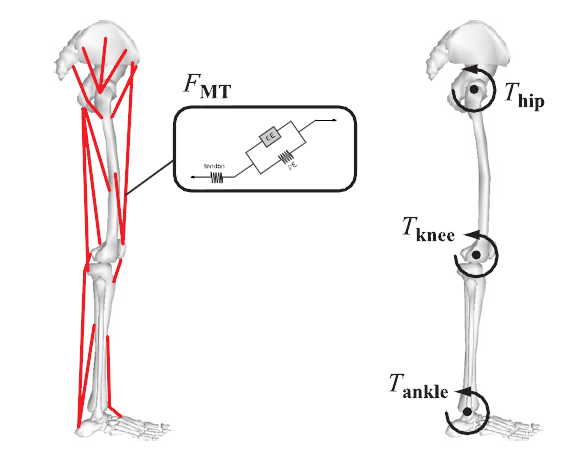
\includegraphics[width=.6\textwidth, height=.30\textheight]{neuromusculoskeletal/fig/muscle-skeleton-torque.png}
    \caption{Συσχέτιση παραγόμενης δύναμης από τον μυ με ροπές στις αρθρώσεις\cite{erdemir07}}
    \label{fig:force-torques}
\end{figure}

\begin{equation}
    R_{ij} = - \frac{\partial L_{j}(q)}{\partial q_{i}}
    \label{equ:muscle-moment-arm}
\end{equation}

Είναι φανερό, ότι υπολογισμός της δύναμης που ασκεί ο μυς είναι απαραίτητη η γνώση της διάταξης την συγκεκριμένη χρονική στιγμή. Κάτι που πρέπει να τονίσουμε είναι ότι κάθε μυς έχει μια συγκεκριμένη γεωμετρία και τυλίγεται με διαφορετικό τρόπο πάνω στον σκελετό. Δεν μπορούμε να θεωρήσουμε ότι ένας μυς απλά ξεκινάει σε ένα σημείο Α και καταλήγει σε ένα άλλο σημείο Β. Είναι απαραίτητη η περιγραφή της διαδρομής που ακολουθεί από μια ακολουθία σημείων, αλλά και τον τρόπο με τον οποίο τυλίγεται στην διάταξη \cite{delp95}. Για να βρεθεί το μήκος του μυ αθροίζονται τα επιμέρους ευθύγραμμα τμήματα που τον δημιουργούν.


